\chapter{Introduction}
\label{ch:Introduction}

Reducing code complexity is a crucial measure in software projects to counteract rising costs for development and maintenance. Nowadays, many applications make use of external components instead of being built completely from scratch. Software reuse increases the productivity of the developers and improves the overall quality of the resulting product. These benefits encourage the popularity of third-party libraries which provide an interface to pretested features, created and maintained by a different team. This public interface of an integrated software component is refered to as its \textit{\ac{API}}. Consumers of an \ac{API} simplify their development effort by taking advantage of the functionality provided without having to worry about its internal implementation, so that they can focus on their own requirements. 

With increasing popularity of distributed systems and the web, APIs have evolved from local libraries to globally available services, providing language-independent access to actions and resources on remote machines which require central coordination or storage.The \ac{W3C} coined the term \textit{Web Service} for services using \textit{\ac{SOAP}} messages that trigger \textit{\acp{RPC}} and are typically transmitted using HTTP with an \acs{XML} serialization\footnote{https://www.w3.org/TR/ws-arch}. Web based services are identified by \textit{\acp{URI}} in either an action-based or resource-based format. Their functionality is described using an \textit{\ac{IDL}} like \textit{\ac{WSDL}} or the OpenAPI Specification. In the remainder of this thesis, \textbf{Web APIs} denote modern, language-agnostic \acp{API}, that are described by \acp{IDL} and can be accessed via HTTP and its standard ports by exchanging non-verbose messages in a human-readable or binary format. We define a verbose format as a messaging format that uses additional elements containing meta information to describe the message content instead of implicitly inferring this information by structure or other means. While, contrary to our definition, Web APIs may be provided on ports other than the standard HTTP ports 80 \& 443, this configuration is predominantly found in productive systems.

 According to ProgrammableWeb\footnote{https://www.programmableweb.com/}, one of the world's largest \ac{API} directories, \acs{REST} is the predominant architectural style for Web APIs with over 14,000 \acp{API} listed, followed by \ac{RPC} with about 1,700 entries. Their directory is currently recording an average monthly increase of 168 entries. With new technologies like GraphQL and gRPC emerging, this number will continue to rise. In addition to the consumers, the providers also benefit from supplying an \ac{API}. They are able to increase their customer reach and create a new revenue stream by monetizing it \cite[p. 243]{koci_classification_2019}. 

Despite their many advantages, using external components has one major drawback regarding their evolution. Software evolution denotes all changes to software systems after the initial release, which can also include architectural changes \cite{eilertsen_exploring_2018}. Eilertsen et. al also note that \ac{API} evolution is closely related to software evolution research and is a fairly new field. Due to the decoupled provision and consumption of APIs, the authors refer to the independent evolution process as co-evolution. 

Since providers can unilaterally introduce changes to API contracts, these can cause build or runtime errors in consuming applications, commonly referred to as breaking changes. The prevalent way for library consumers to handle them, was by not upgrading to the latest version. In contrast to statically linked libraries, web services can neither be rolled back nor can a specific version be used beyond the end of its support. Instead, consumers now have to adapt their applications by manually going through a cumbersome process which is associated with a lot of additional effort. For providers, the upgrading forced on their consumers is no desirable option either. Especially for public providers, who in this case might lose customers to alternative providers \cite[p.3]{lubke_interface_2019}. 


\section{Motivation}
\label{sec:Motivation}

Given the importance of dealing with API evolution, much research has been devoted into this area. Espinha et al. \cite{espinha_web_2014} investigated the challenges for client developers regarding API changes and identified how large providers organize their evolutionary process. In \cite{brito_you_2020}, Brito et al. conducted a field study to determine the motivation of API providers to introduce breaking changes. For a better understanding of Web API evolution, Li et al. \cite{li_how_2013} examined large popular Web APIs and defined common characteristics of changes. Given the recurring features of API changes, Lübke et al. \cite{lubke_interface_2019} extracted a number of patterns for evolving Web APIs from best practices found in major public services as well as in literature. 

Due to the fact that adapting a client application to the latest version of an API is cumbersome, various approaches to automate the migration process have been proposed. However, automation techniques for library evolution such as capturing and replaying refactoring steps \cite{henkel_catchup!_2005} or using twinning to adapt to alternative APIs \cite{nita_using_2010} have been rarely adopted in practice \cite[p. 300]{li_how_2013} and cannot be applied to remote Web APIs. Although tools were created to allow developers to parse IDLs to generate client libraries and server stubs in all modern programming languages, this generated code is a static view of an API and does not support migratory adaptions. Hence, every breaking change is directly reflected in the generated library and breaks the client application. 

Regardless of whether an IDL generator is used to create a library, the workflow remains inconvenient for API consumers. Due to the independent release cycles, API providers update their code and documents without knowing how it might affect their consumers. Breaking changes are not necessarily limited to modifications to the public interface, but can also occur in the event of alterations in internal behavior such as changing standard parameters or return values. As shown in Figure \ref{fig:oldWorkflow}, API consumers may not be notified of a new release and will only find out about it after their application has malfunctioned. 

\begin{figure}[h]
	\centering{
		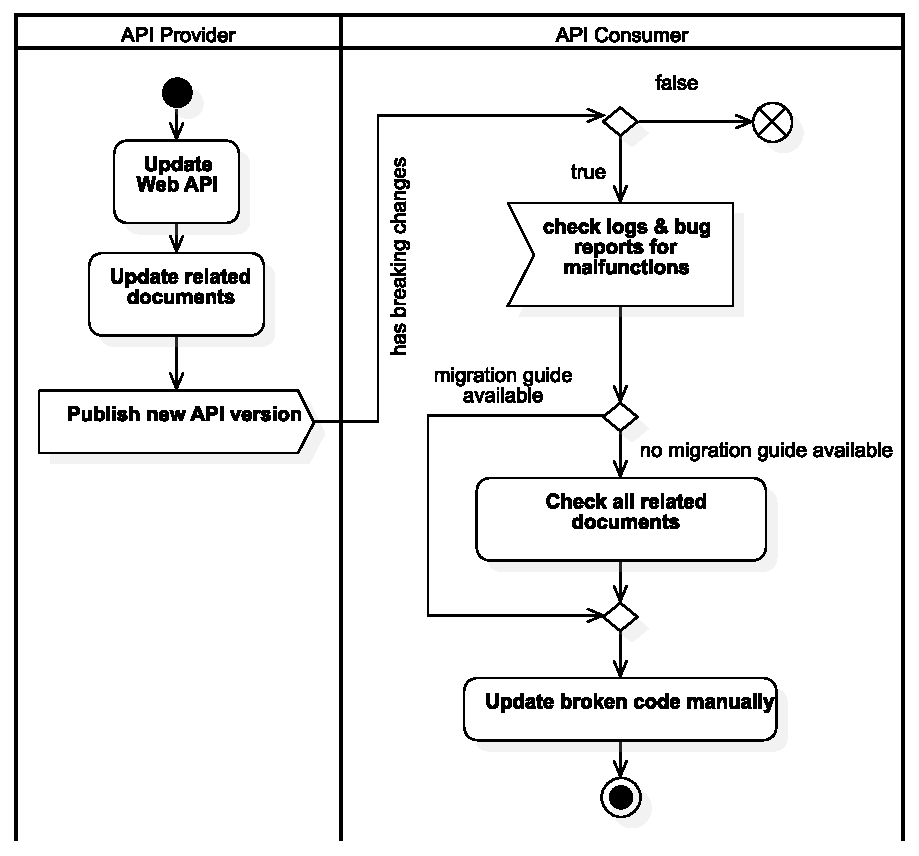
\includegraphics[width=125mm]{images/old_workflow.pdf}
		\caption{Cumbersome workflow after web service changes}
		\label{fig:oldWorkflow}
	}
\end{figure}

In a field study, Brito et. al questioned API providers on how they plan to document their changes. They found out that 22\% usually use release notes or changelogs, while only 11\% aim to provide a migration guide. Without a detailed guide that includes all of the steps required to migrate between versions, API consumers have to go through various documents and apply the modifications themselves. Resolving breaking changes manually is error-prone and leads to rising maintenance costs. A tool-based workflow could significantly shorten the time from detection to the incorporation of changes and thus reduce maintenance costs and errors.

Recent research on API evolution focuses on classifying breaking changes and patterns for Web APIs or adapting client code after updating a local library. Currently, there is a research gap regarding tool-supported workflows for migrating client applications after a Web API introduced breaking changes. Research and tools on Web API evolution have the potential to reduce development and maintenance time, improve quality and reliability of client code and prevent manually introduced bugs during the upgrade process. Automated code migration for API consumers would eliminate the need to manually inspect changes listed in change logs, newsletters, release notes or documentations and adapting the code accordingly. 
\section{Objectives}
\label{sec:Objectives}

In this thesis, we propose a new tool-supported workflow in which client code gets automatically migrated after a web service was modified. We focus on light-weight Web API technologies which can be described by an IDL, such as REST, GraphQL and gRPC. Our main objective is to facilitate the workflow shown in Figure \ref{fig:oldWorkflow} by significantly reducing the effort for API consumers. Therefore, we introduce a state-of-the-art description language to specify a machine-readable migration guide. This guide enables API providers to describe all modifications of a Web API from a previous to its latest version. In addition, we propose a tool that parses our migration guide and generates library code that is persistent to changes to its public interface once it is run for the first time. It can be used in an existing \textit{\ac{CI/CD}} pipeline or via the command line.

\begin{figure}[h]
	\centering{
		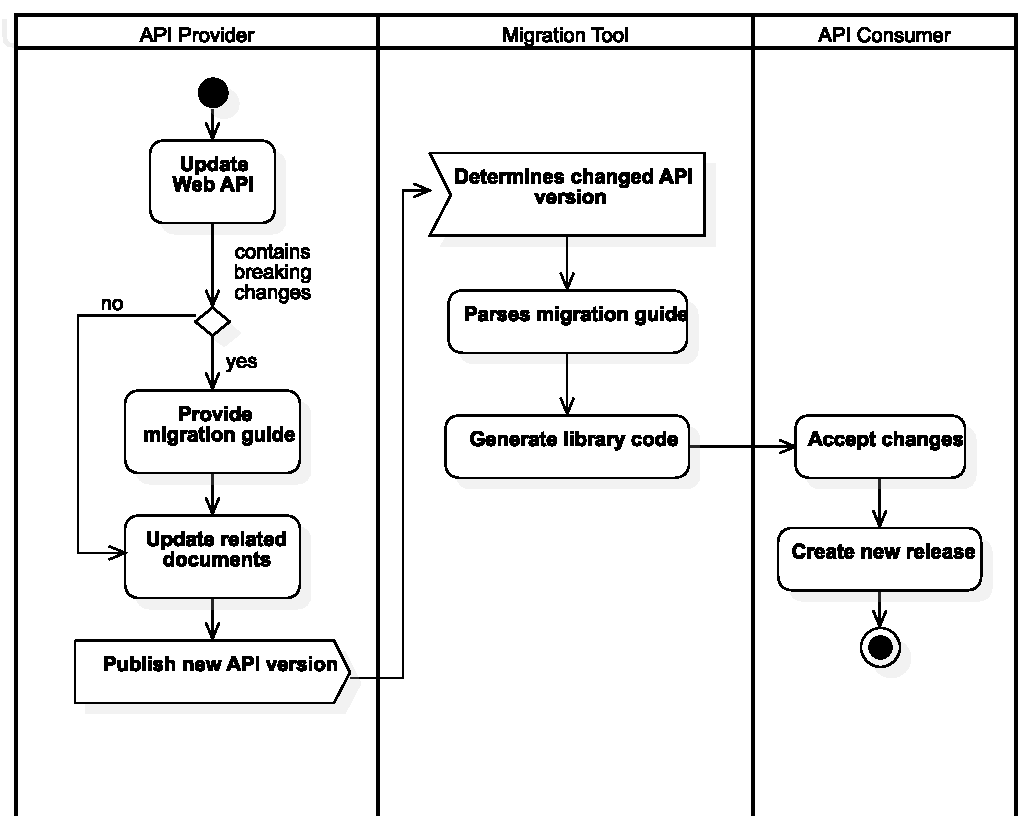
\includegraphics[width=128mm]{images/new_workflow.pdf}
		\caption{Workflow with tool support after web service changes}
		\label{fig:newWorkflow}
	}
\end{figure}

Figure \ref{fig:newWorkflow} showcases the new workflow. In addition to their current tasks, Web API providers must state all introduced changes in a machine-readable migration guide and make it available to consumers. Web API consumers have to integrate our migration tool, which automates the incorporation of changes without breaking the client application. It determines the API version from the migration guide and creates a set of rules indicating how the library should be customized to avoid introducing breaking changes to the consumer's application code. After executing these rules, the public interface of the generated library code remains unchanged and the consumer's application continues to use the library's code which acts as a facade for the lower level API calls.
\section{Outline}
\label{sec:Outline}

After the initial introduction into challenges of Web API evolution and our motivation to overcome them in Chapter \ref{ch:Introduction}, we examine the current state of related research topics in Chapter \ref{ch:RelatedWork}. Identifying the challenges in related research faciliates defining the key requirements for our proposed workflow and discovers several limitations to be aware of as Web APIs evolve. Chapter \ref{ch:RequirementsElicitation} comprises all requirements and constraints we identified from related work. In addition, we were able to derive multiple use cases from potential real-world scenarios. Taking into account all requirements and the existing related work, we create the design of our proposed system, which is described in Chapter \ref{ch:SystemDesign}. Our system is composed of multiple subsystems that each provide their own functionality. In Chapter \ref{ch:ObjectDesign} we select detailed solutions for individual subsystems by identifying either suitable third-party components or pattern templates. We instantiate our proposed system in \textsc{Pallidor}, our prototypical implementation in the Swift programming language. In Chapter \ref{ch:CaseStudyEvaluation}, we use Pallidor to migrate various types of change for a sample Web API and evaluate our proposed system based on our findings. Chapter \ref{ch:Summary} concludes the thesis and discusses future work.